\section{Monte Carlo model of Deep Exclusive $\pi^{-}$ Production from the Neutron in $^{3}He$ }
One of the primary goals of this proposed measurement is to extend our knowledge of the $\sigma_{L}$, $\sigma_{T}$, 
$\sigma_{LT}$ and $\sigma_{TT}$ to larger values of $Q^2$, $-t$ and $W$. Initial Monte Carlo studies require a model for 
experimentally unexplored region of kinematics. The electroproduction of charged pion is best described by the VR model~\cite{vr}.
 A brief description of VR model is given in section 1.2. The scattering cross section for 
$n(e,e^{\prime}\pi^{-})p$ in one-photon exchange is given by equation $\ref{equation:cross-1}$:

\begin{equation}
  \frac{d^{5} \sigma}{dE' d\Omega_{e'} d\Omega_{\pi}} = \Gamma_{V} \frac{d{^2} \sigma}{d\Omega_{\pi}}.
  \label{equation:cross-1}
\end{equation}

The virtual photon flux factor $\Gamma_{V}$ in equation $\ref{equation:cross-1}$ is defined as:

\begin{equation}
  \Gamma_v=\frac{\alpha}{2\pi^2} \frac{E'}{E} \frac{K}{Q^2}\frac{1}{1-\epsilon},
  \label{equation:photon-flux-1}
\end{equation}
where $\alpha$ is the fine structure constant, $K$ is the energy of real photon equal to the photon energy required to create 
a system with invariant mass equal to $W$ and $\epsilon$ is the polarization of
the virtual photon.

\begin{equation}
  K=(W^2-M_p^2)/(2 M_p)
  \label{equation:photon-flux-2}
\end{equation}

\begin{equation}
  \epsilon=\left(1+\frac{2 |\mathbf{q}|^2}{Q^2} \tan^2\frac{\theta_{e}}{2} \right)^{-1},
  \label{equation:photon-flux-3}
\end{equation}

where $\theta_{e}$ is the scattering angle of scattered electron. The two-fold differential cross section 
$\frac{d{^2} \sigma}{d\Omega_{\pi}}$ in the lab frame can be expressed in terms of the invariant cross section in centre of 
mass frame of photon and proton:

\begin{equation}
  \frac{d^2 \sigma}{d\Omega_\pi}= J \frac{d^2 \sigma}{dt d\phi},
  \label{equation:cross-2}
\end{equation}

where $J$ is the Jacobian of transformation of coordinates from lab $\Omega_{\pi}$ to $t$ and $\phi$ (CM). The invariant cross section 
of equation $\ref{equation:cross-2}$ can be expressed in four terms. Two terms correspond to the polarization states of the virtual 
photon (L and T) and two states correspond to the interference of polarization states (LT and TT),

\begin{equation}
  2\pi \frac{d^2 \sigma}{dt d\phi} =  \epsilon  \frac{d\sigma_{\mathrm{L}}}{dt} + \frac{d\sigma_{\mathrm{T}}}{dt} + 
  \sqrt{2\epsilon (\epsilon +1)} \frac{d\sigma_{\mathrm{LT}}}{dt} \cos{\phi} + \epsilon  \frac{d\sigma_{\mathrm{TT}}}{dt} \cos{2 \phi}
  \label{equation:cross-3}
\end{equation}

\subsection{Data Constraints}
\label{dataconstraints}
Precise $L/T$ separated experimental data of exclusive electroproduction of $\pi^{-}$ on $^2$H are available up to $Q^2 = 2.57$ GeV$^2$, 
$-t = 0.350$ GeV$^2$ and $W = 2.168$ GeV \cite{gmhuber-2}. Precise $L/T$ separated experimental data of exclusive electroproduction 
of $\pi^{+}$ on $^1$H are available up to $Q^2 = 2.703$ GeV$^2$, $-t = 0.365$ GeV$^2$ and $W = 2.127$ GeV \cite{gmhuber}. In \cite{hallc-1} 
and \cite{hallc-2}, separated $\sigma_{L}$ and $\sigma_{T}$ are measured up to $Q^2 = 4.703$ GeV$^2$ and $W = 2.2$ GeV. CLAS 
experiment E99-105 measured the unseparated cross section at $Q^2$ up to $4.35$ GeV$^2$ and $-t$ up to $4.5$ GeV$^2$ \cite{park}. 
The HERMES collaboration measured the unseparated cross section for $Q^2$ = 3.44 GeV$^2$ and 5.4 GeV$^2$ \cite{hermes} at $W$ = 4 
GeV. 

\subsection{Model for Higher $Q^2$ Kinematics}
The electroproduction of charged pion is best described by the VR model \cite{vr}. The VR model is a 
Regge model with a parametrization of deep inelastic scattering amplitude to improve the description of $\sigma_{T}$. The 
description of $\sigma_{L}$ is constrained by a fit to our $F_{\pi}$ data from JLab~\cite{gmhuber}. In figure $\ref{fig:expvrfit}$ we plotted the 
last six data points of table $v$ of \cite{gmhuber-2}, our parametrization and VR model points for exactly same 
values of $Q^2$, $-t$ and $W$. It shows the comparison of the same points of $\sigma_{L,T,LT,TT}$ vs. $Q^{2}$. 

\begin{figure}[!hbt]
    \centering
    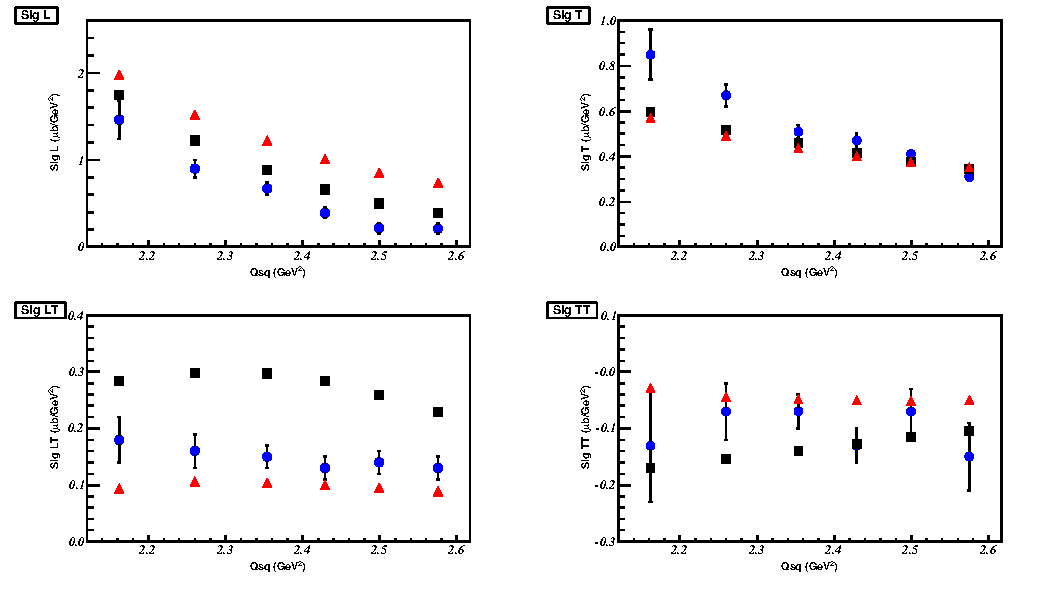
\includegraphics[width=6.0in,height=2.4in]{./figures/pimsigma_qsq.pdf}
    \caption{ A comparison of last six points of table $v$ of ~\cite{gmhuber-2}, VR model and our parametrization values vs. $Q^{2}$ 
    of $\pi^{-}$ electroproduction. Experimental data is shown in blue circles, VR model is shown in red triangles and our 
    parametrization is shown in black boxes. In each graph value of $-t$ is decreasing left to right from maximum value 0.35 GeV$^2$ 
    to 0.15 GeV$^2$. Value of $W$ also decreases left to Right from 2.2978 GeV to 2.1688 GeV.}
    \label{fig:expvrfit}
\end{figure}

\subsection{Parametrization of $\sigma_{L}$, $\sigma_{T}$, $\sigma_{LT}$, $\&$ $\sigma_{TT}$}
\label{parametrization}
For exclusive DEMP in SoLID the kinematic region of interest for parametrization of $\sigma_{L,T,LT,TT}$ is $Q^2$ 
from $4.5$ GeV to 7.5 GeV, $-t$ from 0 GeV$^2$ to 1.0 GeV$^2$ and we set $W=3.0$ GeV. After the parametrization of 
$\sigma_{L,T,LT,TT}$ for $-t$ and $Q^2$, we used the same $W$ dependence given by ~\cite{gmhuber} which is $(W^2-M^2)^{-2}$ where
$M$ is the proton mass. Our parametrization of all four cross sections is given in equations $\ref{equation:l-fit}$ to 
$\ref{equation:tt-fit}$:

\begin{equation}
        \sigma_{L} = \exp{(P_1(Q^2) + |t| * P^{\prime}_1(Q^2))} + \exp{(P_2(Q^2) + |t| * P^{\prime}_2(Q^2))}
     \label{equation:l-fit}
\end{equation}

\begin{equation}
        \sigma_{T} =  \frac{\exp{(P_1(Q^2) + |t| * P^{\prime}_1(Q^2))}}{P_{1}(|t|)}
     \label{equation:t-fit}
\end{equation}

\begin{equation}
        \sigma_{LT} = P_{5}(t(Q^2))        
     \label{equation:lt-fit}
\end{equation}

\begin{equation}
        \sigma_{TT} = P_{5}(t(Q^2)),        
     \label{equation:tt-fit}
\end{equation}

where the parameters $P_{i}$ are polynomial functions of $ith$ order. Each coefficient ($P_{i}$) of fifth order equations 
$\ref{equation:lt-fit}$ and $\ref{equation:tt-fit}$ is a further second order polynomial of $Q^2$. Deep exclusive $\pi^{-}$ events are 
generated using a C++ code. The quality of parametrization is checked by plotting the parametrization functions of $\sigma_{L,T,LT,TT}$ 
versus the VR model as shown in figure $\ref{fig:sigall}$.

\begin{figure}[!hbt]
    \centering
    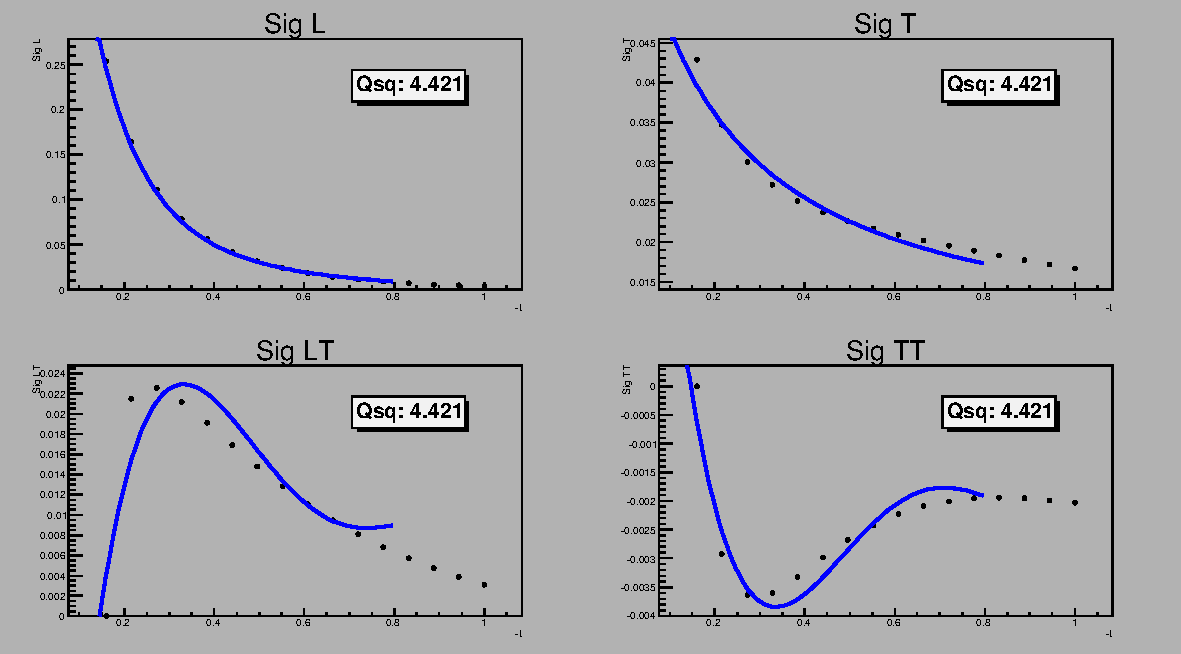
\includegraphics[width=6.0in,height=2.4in]{./figures/pimFit.pdf}
    \caption{ A comparison of parametrized $\sigma_{L,T,LT,TT}$ and VR model values at $Q^2$ = 4.421 GeV$^2$ and $W = 3.0$ GeV.  
    Black points are VR model values and blue line is parametrized $\sigma_{L,T,LT,TT}$ given by equations 
    $\ref{equation:l-fit}$ to $\ref{equation:tt-fit}$. }
    \label{fig:sigall}
\end{figure}

Figure $\ref{fig:sigall}$ shows the comparison of parametrization of $\sigma_{L,T,LT,TT}$ and VR model points. The blue line is the 
parametrization curve and black points are the VR model points.

\subsection{Single Spin Asymmetry (SSA) $\bf{A_{L}^{\perp}}$ }
\label{singlespinasymmetry}
It is shown in \cite{frankfurt} that the generalized parton distribution ($\tilde{E}$) can be probed by measuring the single spin 
asymmetry$(SSA)$. The SSA is defined in equation $\ref{equation:ssa}$, where $\beta$ is the angle between the transversely polarized 
target vector and the reaction plane, and $\sigma_{L}^{\pi^{-}}$ is the exclusive $\pi^{-}$ cross section for longitudinal virtual photons. 
We parametrized the single spin asymmetry using the model of \cite{frankfurt} at $x = 0.1$ and $x = 0.3$. Parametrization of $SSA$ 
is shown in Figure $\ref{fig:asym-1}$ and equation $\ref{equation:asy-fit}$ is the parameterized function of single spin asymmetry.

\begin{equation}
  \bf{A_{L}^{\perp}} = \frac{\int^{\pi}_{0}d\beta\frac{d\sigma_{L}^{\pi^{-}}}{d\beta} - \int^{2\pi}_{\pi}d\beta\frac{d\sigma_{L}^{\pi^{-}}}{d\beta} } 
       {\int^{2\pi}_{0}d\beta\frac{d\sigma_{L}^{\pi^{-}}}{d\beta}}         
     \label{equation:ssa}
\end{equation}

\begin{equation}
        \bf{A_{L}^{\perp}} = \left\{
        \begin{array}{rl}
        A_{0} \left[ 1 - \exp^{ [ -\lambda \times ( t - t_{min} ) ] } \right] & \text{if } t \ge t_{min}, \\
        0 &  \text{if } t < t_{min}.
        \end{array} \right.
     \label{equation:asy-fit}
\end{equation}

\begin{figure}[!hbt]
    \centering
    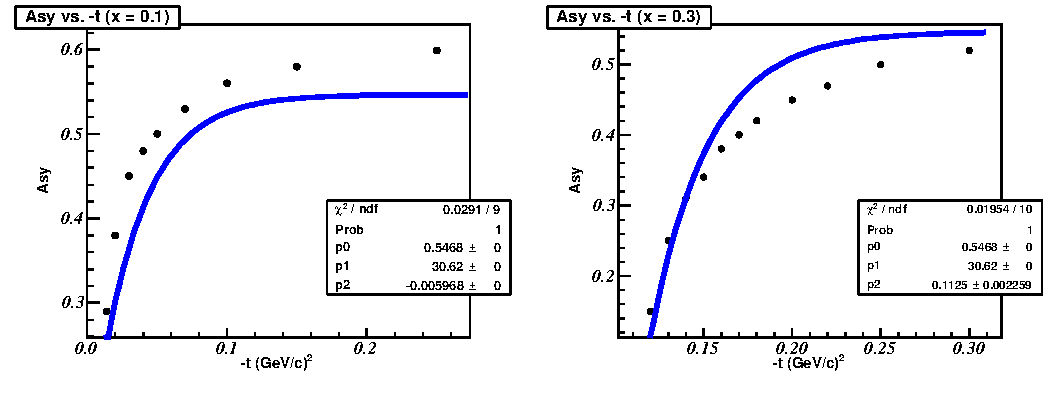
\includegraphics[width=6.0in,height=1.45in]{./figures/asym_3.pdf}
    \caption{ Parametrization of single spin asymmetry $\bf{A_{L}^{\perp}}$ vs. $-t$ at $Q^2$ = 10 GeV$^2$ in 
    left graph $x = 0.1$ and in right  graph $x = 0.3$ where the points are from the model defined in \cite{frankfurt} 
    and blue line is our parametrization function.}
    \label{fig:asym-1}
\end{figure}

\subsection{ Target Neutron Fermi Momentum }
\label{fermimotion}
A histogram of the spectral function of $^3$He is shown in Fig. $\ref{fig:fermi}$ , generated according to Ref. 
\cite{fermipaper}. Neutron momenta up to 300 MeV/c are generated according to this distribution, uniformly distributed in 
spherical coordinates. The quasi-free collision between virtual photon and moving neutron is then transformed to the 
fixed neutron frame, after which the parameterizations of Secs. $\ref{parametrization}$, $\ref{singlespinasymmetry}$ are 
applied. The outgoing particles are then transformed back to the lab frame for tracking.

\begin{figure}[!hbt]
    \centering
    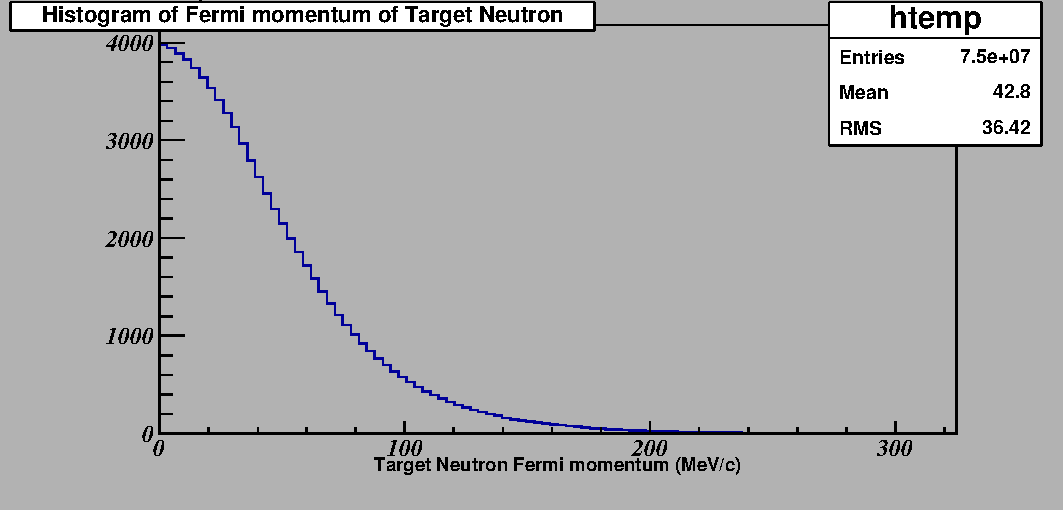
\includegraphics[width=4.0in,height=2.5in]{./figures/Fermi.pdf}
    \caption{Fermi momentum spectral function of a target nucleon in $^3$He generated according to the Argonne 
    potential of Ref \cite{fermipaper}.  The horizontal axis is nucleon momentum in MeV/c.}
    \label{fig:fermi}
\end{figure}
\subsection{Energy Loss}
Energy losses via ionization and Bremsstrahlung have been taken into account for incoming Electrons, scattered Electrons, and Pions, as well as
recoil Protons when they travel through the air and the target. Bremsstrahlung and Ionization losses are calculated according to functions defined in SAMC~\cite{samc}. 
Energy and momentum of these particles are corrected after energy losses.